\documentclass[12pt]{article}

\usepackage[margin=1in]{geometry}
\usepackage{setspace}
\onehalfspacing
\usepackage{graphicx}
\graphicspath{report_images/}
\usepackage{appendix}
\usepackage{listings}
\usepackage{float}
\usepackage{multirow}
\usepackage{amsthm}
% The next three lines make the table and figure numbers also include section number
\usepackage{chngcntr}
\counterwithin{table}{section}
\counterwithin{figure}{section}
% Needed to make titling page without a page number
\usepackage{titling}

% DOCUMENT INFORMATION =================================================
\font\titleFont=cmr12 at 11pt
\title {{\titleFont ECEN 410:  Linear Control System \\ North Carolina Agricultural and Technical State University \\ Department of Electrical and Computer Engineering \\ Dr. Christopher Horne}} % Declare Title
\author{\titleFont  Chris Cannon} % Declare authors
\date{\titleFont November 29, 2018}
% ======================================================================

\begin{document}

\begin{titlingpage}
\maketitle
\begin{center}
	Exam 2 Research Paper
\end{center}
\end{titlingpage}

\tableofcontents

\pagebreak

\section{Introduction}

This paper provides analysis of a control system of the azimuth position of an antenna. This is a critical controls problem in today's world, where immediate access to information is considered an absolute necessity. Emergency response personnel, military entities, other government organizations, and even private citizens depend upon immediate access to information in critical situations every day. This analysis will focus on the response of the system to various inputs, by determining the transfer function of each subsystem as well as the system as a whole.

\begin{figure}[H]
\begin{center}
	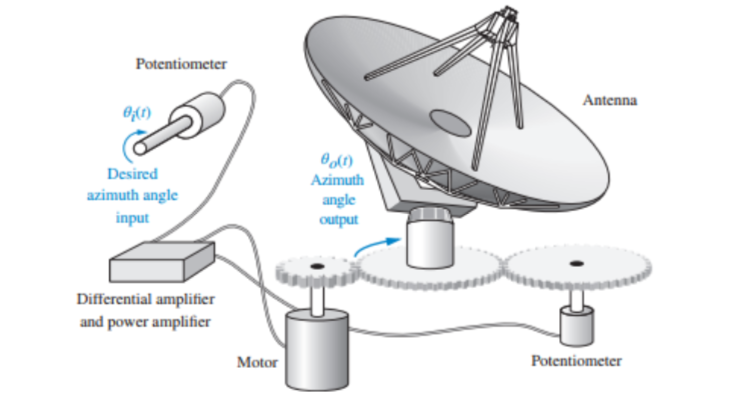
\includegraphics[width=0.8\textwidth]{./img/SystemLayout.png}
	\caption{\label{fig:SysLayout}Control system layout}
\end{center}
\end{figure}

\begin{figure}[H]
\begin{center}
	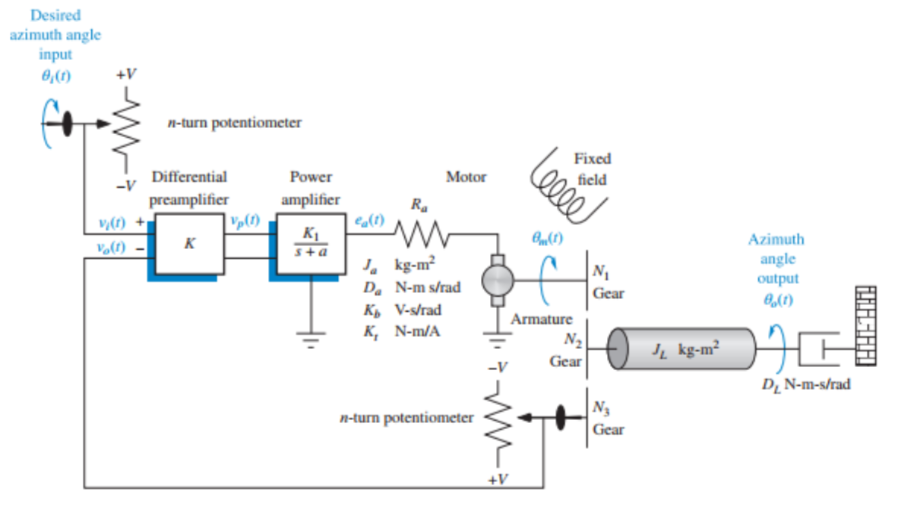
\includegraphics[width=0.8\textwidth]{./img/SystemSchematic.png}
	\caption{\label{fig:SysSchematic}Control system schematic}
\end{center}
\end{figure}

\begin{figure}[H]
\begin{center}
	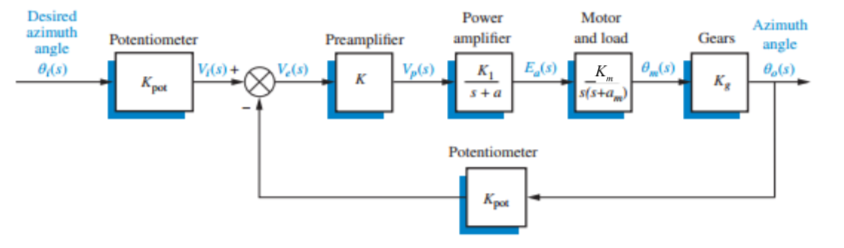
\includegraphics[width=0.8\textwidth]{./img/SystemBlockDiagram.png}
	\caption{\label{fig:SysBlockDiagram}Control system block diagram}
\end{center}
\end{figure}

\subsection{Assumptions}

There are several assumptions that must be made in order to complete this analysis. My general assumptions for the parameters are summarized in Table ~\ref{tab:assumptions} below.

\begin{table}[H]
\begin{center}
\begin{tabular}{| l | l |}
	\hline
	Parameter & System \\ \hline
	\textit{K\textsubscript{pot}} & 0.318 \\ \hline
	\textit{K} & 1 \\ \hline
	\textit{K\textsubscript{l}} & 100 \\ \hline
	\textit{a} & 100 \\ \hline
	\textit{K\textsubscript{m}} & 2.083 \\ \hline
	\textit{a\textsubscript{m}} & 1.71 \\ \hline
	\textit{K\textsubscript{g}} & 0.1 \\ \hline
\end{tabular}
\caption{\label{tab:assumptions}Assumptions made for analysis of the system \cite{nise}}
\end{center}
\end{table}

For this analysis, I also make the following assumptions:
\begin{itemize}
	\item There is no disturbances or interference in the signals between subsystems.
	\item "Motor" in the system is an armature controlled DC servo motor.
\end{itemize}

\section{Analysis}

Analysis will be supplemented with MatLab to plot the relationships between system inputs, outputs, and gains.

\subsection{Potentiometer}

The input potentiometer is used by the user to input a desired azimuth angle $\theta$ for the system.

\begin{figure}[H]
\begin{center}
	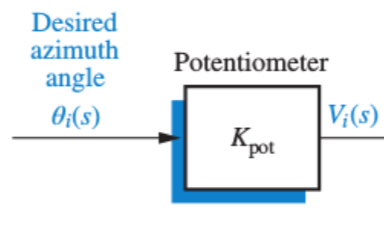
\includegraphics[width=0.3\textwidth]{./img/PotentiometerBlock.png}
	\caption{\label{fig:pot}Input Potentiometer}
\end{center}
\end{figure}

From Figure ~\ref{fig:pot} above, I observed that the transfer function for the input potentiometer subsystem is the potentiometer output $V_{i}(s)$ divided by the user entered azimuth angle $\theta_{i}(s)$. Therefore:

\begin{equation}
\frac{V_{i}(s)}{\Theta_i(s)} = K_{pot}\label{eq:1}
\end{equation}

Based on the Equation ~\ref{eq:1} above, and the previously stated assumption that $K_{pot} = 0.318$, I am able to plot the transfer function for the input potentiometer. I analyzed the transfer function in the time domain using plots of the step and impulse responses. For frequency domain analysis, I used Nyquist and bode plots. These plots helped me determine gain and phase in the frequency domain.

%TODO add potentiometer plots here

\subsection{Preamplifier}

The preamplifier is shown in Figure ~\ref{fig:preamp} below.

\begin{figure}[H]
\begin{center}
	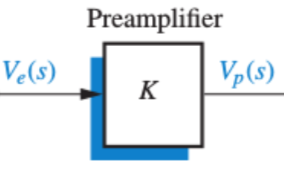
\includegraphics[width=0.3\textwidth]{./img/PreamplifierBlock.png}
	\caption{\label{fig:preamp}Preamplifier}
\end{center}
\end{figure}

As with the potentiometer, I can determine by inspection that the transfer function of the preamplifier is equal to the output divided by the input. Therefore:

\begin{equation}
\frac{V_{p}(s)}{V_{e}(s)} = K\label{eq:2}
\end{equation}

Using my assumptions above that $K = 1$, once again I plotted the step and impulse responses, as well as the Nyquist and bode plots.

%TODO add preamp plots here

\subsection{Power Amplifier}

The power amplifier subsystem is shown in Figure ~\ref{fig:amp} below.

\begin{figure}[H]
\begin{center}
	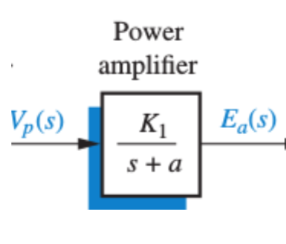
\includegraphics[width=0.3\textwidth]{./img/PowerAmplifierBlock.png}
	\caption{\label{fig:amp}Power Amplifier}
\end{center}
\end{figure}

Once again using inspection, I found the transfer function for the amplifier to be:

\begin{equation}
\frac{E_{a}(s)}{V_{p}(s)} = \frac{K_{1}}{s+a}\label{eq:3}
\end{equation}

Based on assumptions above, $K_{a} = a = 100$. Once again I will use the step and impulse responses, bode and Nyquist plots.

%TODO add amp plots here

\subsection{Motor and Load}

The motor and load subsystem is shown in Figure ~\ref{fig:motor} below.

\begin{figure}[H]
\begin{center}
	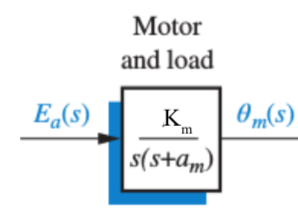
\includegraphics[width=0.3\textwidth]{./img/MotorBlock.png}
	\caption{\label{fig:motor}Motor and Load}
\end{center}
\end{figure}

By inspection, I found the transfer function of this subsystem to be:

\begin{equation}
\frac{\theta_{m}(s)}{E_{a}(s)} = \frac{K_{m}}{s(s+a_{m})}\label{eq:4}
\end{equation}

In Equation ~\ref{eq:4} above, $K_{m}$ is assumed to equal 2.083, and $a_{m}$ is assumed to be 1.71. Using the equation and the previously stated assumptions, I created step and impulse response plots, and well as bode and Nyquist plots.

%TODO add motor plots here

\subsection{Gears}

The block diagram of the gears subsystem is found in Figure ~\ref{fig:gears} below. Note that that feedback for the system also is part of the output of this subsystem.

\begin{figure}[H]
\begin{center}
	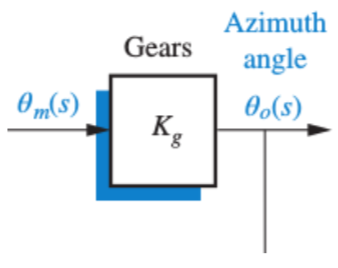
\includegraphics[width=0.3\textwidth]{./img/GearsBlock.png}
	\caption{\label{fig:gears}Gears}
\end{center}
\end{figure}

Using inspection, the transfer function for this subsystem is as follows:

\begin{equation}
\frac{\theta_{o}(s)}{\theta_{m}(s)} = K_{g}\label{eq:5}
\end{equation}

In Equation ~\ref{eq:5} above, I assume that $K_{g} = 0.1$. I again found the step and impulse responses, and bode and Nyquist plots.

%TODO add gears plots here

\subsection{Complete System}

Based on my analysis of the plots in Sections ~\ref{subsec:Potentiometer} through ~\ref{subsec:Gears} above, I can see that the transfer functions of the potentiometers, preamplifier, and gears all remain constant over time. This is all based on the fact that my analysis of the system takes place under a limited set of conditions, mainly $K_{pot}$. If $K_{pot}$ changed, so too would the associated transfer functions.

To determine the overall transfer function of the system, I utilized MatLab.

\section{Conclusion}

\pagebreak

\textbf{Appendices}

\begin{appendices}


\end{appendices}

\begin{thebibliography}{9}

\bibitem{nise}
  Norman S. Nise,
  Control Systems Engineering,
  John Wiley and Sons, New York, New York,
  7th edition,
  2015.

\end{thebibliography}
\end{document}